%!TEX root = ../thesis.tex
%*******************************************************************************
%*********************************** Introduction *****************************
%*******************************************************************************

\chapter{Introduction}
\label{chap:introduction}
\ifpdf
    \graphicspath{{Chapters/Introduction/Figs/}{Chapters/Introduction/Figs/}{Chapters/Introduction/Figs/}}
\else
    \graphicspath{{Chapters/Introduction/Figs/}{Chapters/Introduction/Figs/}}
\fi
In this thesis, we explain our approach to improving \ac{ui} prototyping and \ac{ui} experimentation.
This chapter motivates the readers about the topic (see section~\ref{introduction:section:motivation}), explains the problems faced by the companies during software development (see section~\ref{introduction:section:problems}), our research approach (see section~\ref{introduction:section:research}), and finally, our solution approach (see section~\ref{introduction:section:solution}).

%********************************** % Motivation  **************************************
\section{Motivation} % Section - 1.1 
\label{introduction:section:motivation}

Over the last decade, software development had a tremendous impact with increasing customer demand and requirements \cite{article:swdemand:ahmed}, further increasing product complexity and ambiguity, significantly impacting software development.  
Therefore, the developers have come up with different techniques to meet this requirement criteria.
Early user feedback from potential customers in the industry is crucial for creating successful software products because of the growing market uncertainties, and consumers' desire to receive integrated solutions to their issues rather than unique software developments \cite{misc:businessmodels:teece}.
With the increasing complexity of products, it becomes challenging to determine user requirements making it more difficult for developers to assess their opinions.
As a result, the developers of these products are biased toward some requirements and can ignore what the user wants. 
So, the developers must detect the user's needs and requirements to reduce these risks early.
Giving users a ``partially functioning'' system is the most excellent method to determine their requirements and suggestions \cite{journal:prototyping:davis}.
This ensures that the developers with high uncertainties in the early product development phase can improve the product by testing the underlying assumptions \cite{misc:lean:steve}.
Developers can use this feedback to validate the most critical assumptions about the software product. 
This validation can decide whether to add, remove or update a feature \cite{article:experiments:lindgren}. 
This process of determining the best fit for the product through user feedback is called experimentation.
There has been an increase in interest in the types of experimentation that can take place in product development. 
Software products have shown the benefits of conducting experiments in many use cases with incremental product improvement \cite{article:controlled:experiements}.
In experimentation, the product designers design different UI variants (e.g., buttons with different colors), and the developer integrates these variants and assigns them to a distinct group of users. 
As per some evaluation criteria (e.g., more clicks on the button), the variant with better results is deployed for the entire set of users.
So, an experiment can be valuable when it improves the software products.
Hence, for experiments to be successful, they should offer one or more solutions that will benefit users.

%********************************** % Problem Statement  *************************************
\section{Problem Statement} % Section - 1.2
\label{introduction:section:problems}
The motivation section shows some gaps in software development between the developers and the designers.
This section explains the problems and determines their research and solution approach.

\paragraph{Problem 1:} Product designers create many UI prototypes, and the developers implement them.
To determine the best variant, the developers create experiments with the users \cite{article:experiments:lindgren}. 
This concrete implementation of designs uses a lot of resources and time for the developers.
Therefore, the product designers need to be integrated into the development process so that they would be able to create experiments independent of the developers.

\paragraph{Problem 2:} When the product designers develop the prototypes, testing them with many users is difficult as the product is still not developed.
Therefore, it is not easy to conclude a ``winner'' variant with a small amount of data as it is statistically difficult to prove one of the variants outperforms the others \cite{article:usability:smalldata}.
Therefore, it is necessary to develop an idea that the designers can use to determine the best prototype or variant with a small group of users.

\paragraph{Problem 3:} Most often, the software application collects data from the experiments. 
Some data is used in qualitative analysis, while others are in quantitative analysis.
Many companies fail to reap the benefits of using both qualitative and quantitative analysis.
Similarly, not all the data is used in the analysis phase reducing the software applications to improve based on customer feedback \cite{article:datadrive:brian}.
Therefore, finding a solution that combines qualitative and quantitative data analysis is necessary.

%********************************** % Research Approach  *************************************
\section{Research Approach}  % Section - 1.3 
\label{introduction:section:research}
The process of creating experiments and testing their variants is usually not systematically arranged, creating anomalies, and leading to unsuccessful experiments.
Therefore, this section identifies the \ac{rq} and defines an approach to answer the question.

\paragraph{\ac{rq}:} \textit{How to develop software suitable for product designers to conduct experiments on UI prototypes, increasing its usability and, simultaneously, independent of developers?}\\

\begin{figure}[ht]
    \centering
    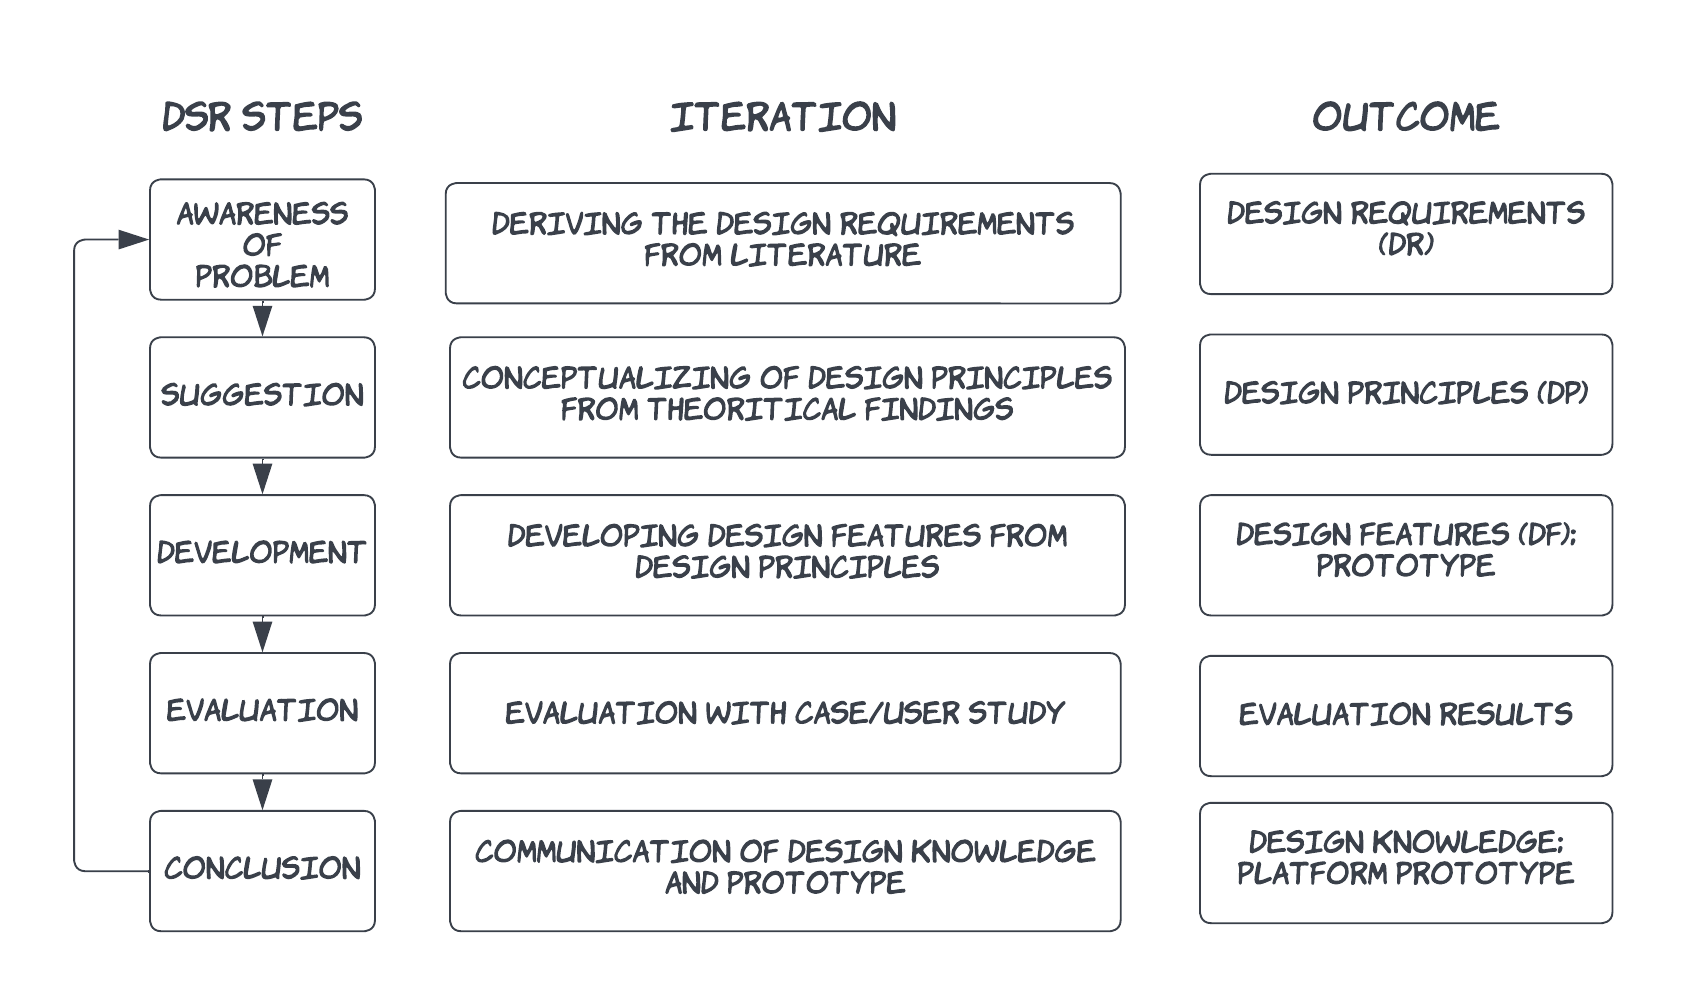
\includegraphics[scale=0.2]{DSRcycle.png}
    \caption[Design Science Research Cycle]{Design Science Research Cycle \cite{paper:designprinciple:vk}}
    \label{intro:fig:dps}
\end{figure}

Prescriptive knowledge about the design of artifacts, such as software techniques, models, or concepts, is what \ac{dsr} aims to provide.
Due to this design knowledge, future projects can design artifacts methodically and scientifically with the aid of study and practice \cite{paper:designprinciple:vk}. 
Therefore, we will conduct the \textit{first} iteration of the \ac{dsr} study to answer our research question and obtain abstract design knowledge and an implementation tool. 
From the abstracted knowledge, we will obtain some \ac{dp} defined for the whole process of experimentation \cite{paper:designprinciple:vk}.
In this design, the product designers will iteratively validate their prototypes with the users or the participants. 
Here, \ac{dp}s capture and codify that knowledge by focusing on the implementer, the aim, the user, the context, the mechanism, the enactors, and the rationale \cite{paper:designprinciple:gregor}. 
The \ac{dp}s explain the design information that develops features for software applications.
We propose to use the variation of the cycle of Kuechler and Vaishnavi \cite{paper:designprinciple:vk} consisting of five iteratively conducted steps (see figure \ref{intro:fig:dps}). 
% First, we identify the 
% \texttt{(1) Awareness of the Problem} and provide a
% \texttt{(2) Suggestion of a possible solution}. Next, we work on the 
% \texttt{(3) Development of the software artifact} and conduct an 
% \texttt{(4) Evaluation} of it. Based on the evaluation results, we provide 
% \texttt{(5) Conclusions} \cite{misc:crowdsourcing:sg}.
% From each step of the DSR, we have an iteration cycle and an outcome (e.g., Awareness of the Problem leads to finding Design Requirements, Design Principles (DPs) can be found from the Suggestion of the solution, Development of the software artifact leads to finding the Design Features and the Prototype, etc.) as shown in figure \ref{intro:fig:dps}.
As a result, this design and application may provide design-focused information that adds to the DSR knowledge corpus \cite{misc:dsr:henver}.
Every element within a DSR project is built upon and systematically analyzed to add to the overall DSR knowledge corpus.
Therefore through the use of \ac{dsr}, a group of issues is resolved by concentrating on a single issue and abstracting the consequences of the resolution.

\paragraph*{Design Requirements:}
In \ac{dsr}, abstracted \ac{dr} refer to the general, high-level requirements that a design must meet to succeed \cite{misc:dsr:webster}. 
These requirements are typically derived from the RQ identified as relevant to the problem.
Abstracted \ac{dr}s provide a broad framework for the design process and help to ensure that the design solution addresses the key issues and challenges identified in the research problem. 
They can also help guide the evaluation of the design solution and ensure that the solution is grounded in the design principles identified as necessary.

\paragraph*{Design Principles:}
In \ac{dsr}, concrete \ac{dp}s refer to specific, detailed guidelines that a design must follow to be successful \cite{misc:dsr:webster}. 
These principles are derived from the abstract \ac{dr}s identified as relevant to the research problem and provide more specific guidance on how the design should be implemented.
DPs can also be defined as the codification of our knowledge during the design study while identifying the DRs. 
Concrete DPs are essential in DSR as they help ensure that the design solution meets the needs and goals of the research problem and is grounded in the \ac{dp}s we identified as necessary.

\paragraph{Design Features:}
In \ac{dsr}, \ac{df} refer to the characteristics of the artifacts or solutions created through the process \cite{misc:dsr:webster}. 
These \ac{df}s provide a means of evaluating the solution's effectiveness and can serve as guidelines for others who may want to adopt or modify the solution.
\ac{df}s typically include both functional and non-functional aspects of the solution. 
Functional features relate to the specific capabilities and functionalities that the solution provides whereas, non-functional features relate to characteristics such as usability, scalability, etc. 
By explicitly specifying these \ac{df}s, DSR researchers can ensure that their solutions are aligned with the stakeholders' needs and meet the necessary standards of quality and effectiveness.

\clearpage
\section{Solution Approach}
\label{introduction:section:solution}

To solve the problems mentioned above, the designers should be able to create UI prototypes and experiments on their own on a set of users.
Since we do not have a large set of users for testing the prototypes, we use supervised task-based usability testing \cite{article:dataanalysis:supervisedtest}.
The fundamental principle of task-based usability testing is to have the users attempt to use the prototypes to do certain activities or tasks (e.g., Locate a movie M1) and get feedback (e.g., the time required for the task to be completed by the user).
We propose to use a low-code or no-code approach to achieve this.
This approach helps to have a UI for the designers to understand, develop, and create experiments and tasks with the software prototypes \cite{paper:lowcode:khorram}.
So, the designers would be able to create the UI prototypes and their variants, assign them to the users in an experiment, get feedback from the users and decide on the best prototype.
At the same time, the low-code has become more accessible for model-driven development \cite{article:lowcode:modeldriven}.
Therefore, we plan to create models for the UI prototypes and have the feasibility for creating experiments and tasks. 
Because of using the models, it is easier to store the prototypes in the database and conduct experiments with the users. 

\begin{figure}[ht]
    \centering
    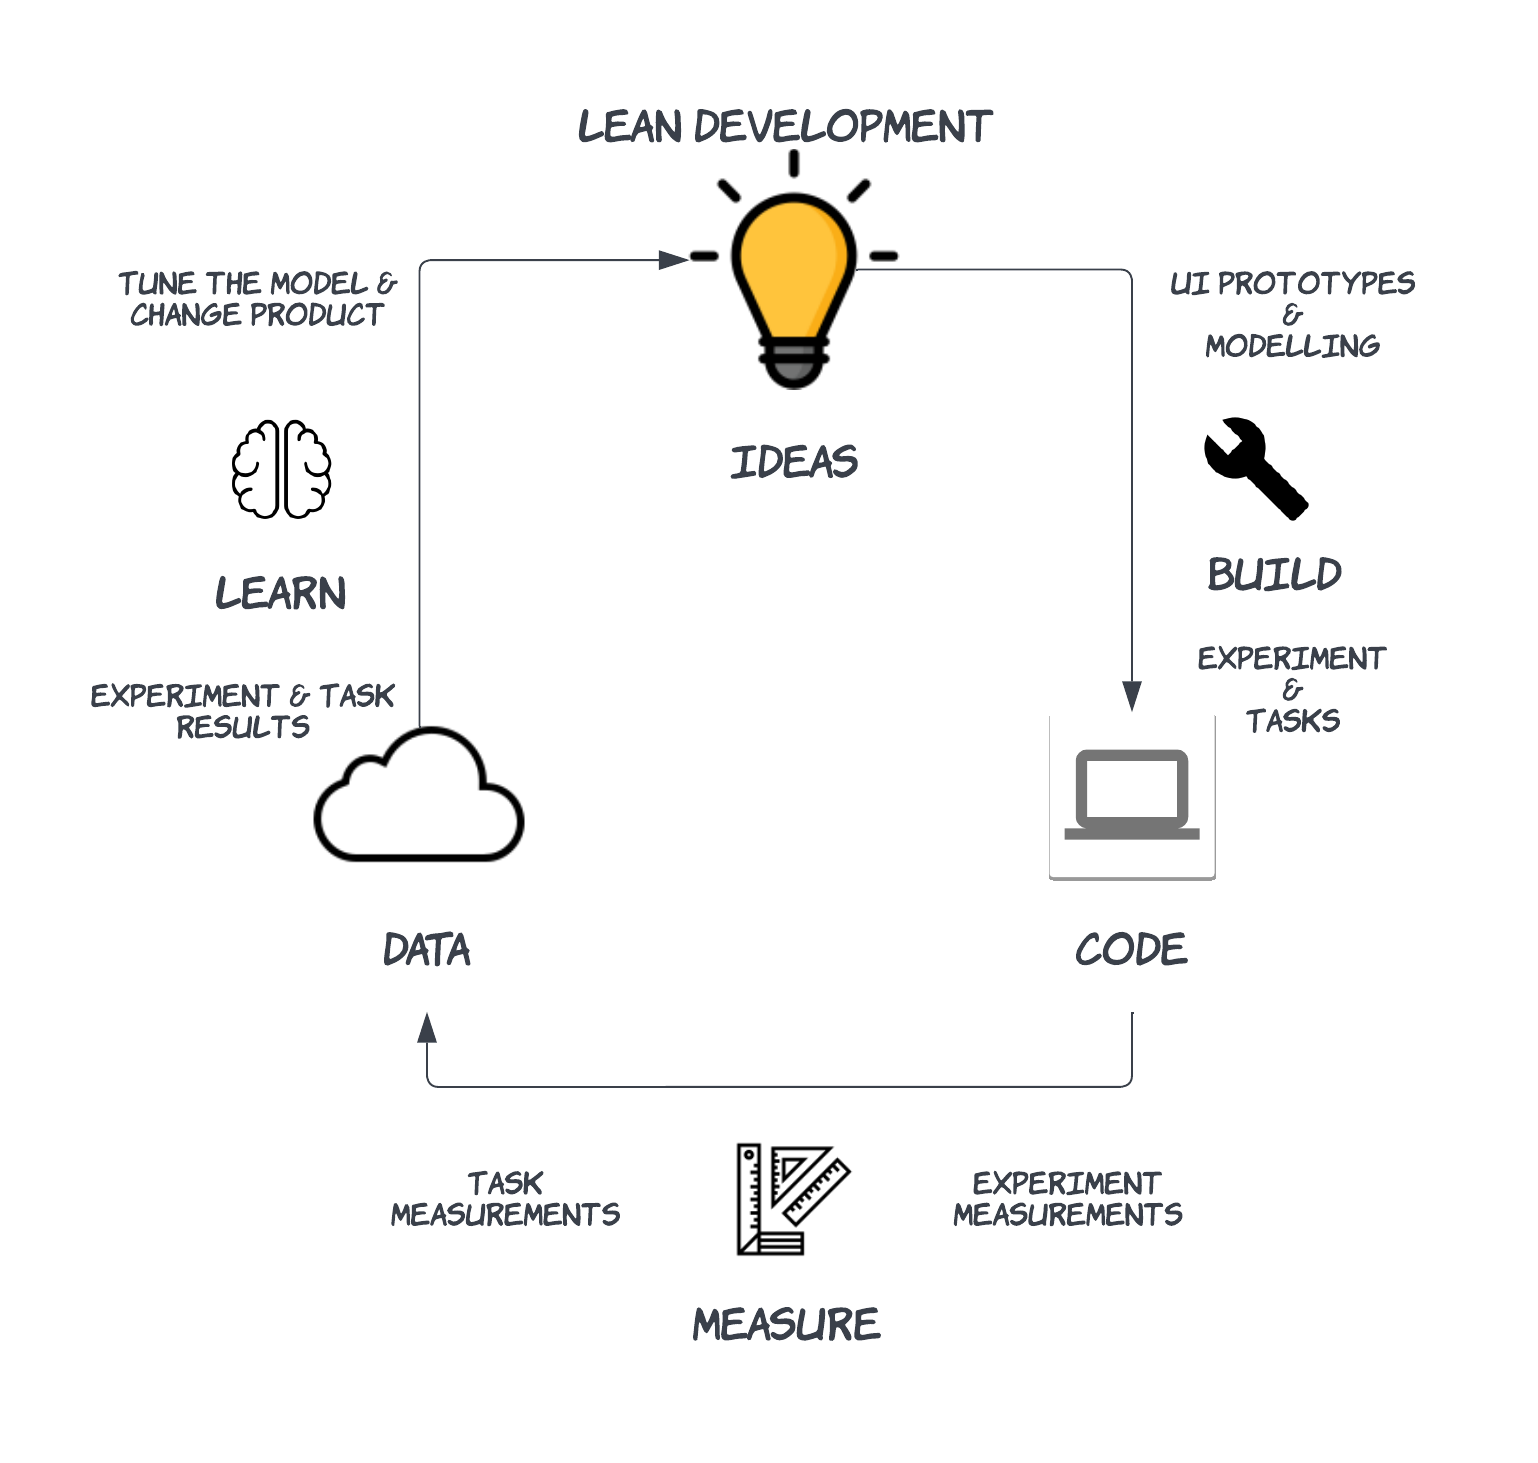
\includegraphics[scale=0.15]{LEAN.png}
    \caption{LEAN Development Technique}
    \label{intro:fig:lean}
\end{figure}

In our solution, we use the LEAN development technique (see figure \ref{intro:fig:lean}) for development as it is used to develop user-friendly products \cite{article:lean:hart}.
Using LEAN, the company creates a Minimum Viable Product (MVP) throughout development, tests it with potential customers, and leverages their input to make incremental changes.
While this technique can be used for every product, there are also approaches specific to software products.
LEAN development technique can be divided into a Build, Measure, and Learn cycle. 
In the \textit{(1) Build} phase, we plan to create the UI prototypes, models, UI experiments, and user tasks.
In the \textit{(2) Measure} phase, we plan to assign the experiments and tasks to the users and measure the task and the experimental measurements and perform some analysis on the data received. 
And finally, in the \textit{(3) Learn} phase, we display the analysis results, tune our models to decide the better variant among the others and modify the prototype.
As per figure \ref{intro:fig:lean}, we complete one cycle of iteration and start a new one with the updated prototype.

\clearpage

\section{Thesis Structure}
The structure of our thesis is designed to provide a comprehensive overview of our research and solution approach.
The \textit{\hyperref[chap:introduction]{(1) Introduction}} chapter includes a detailed analysis of the problem statement, motivation, research question, and our research and solution approach.

\begin{figure}[htbp!]
    \centering
    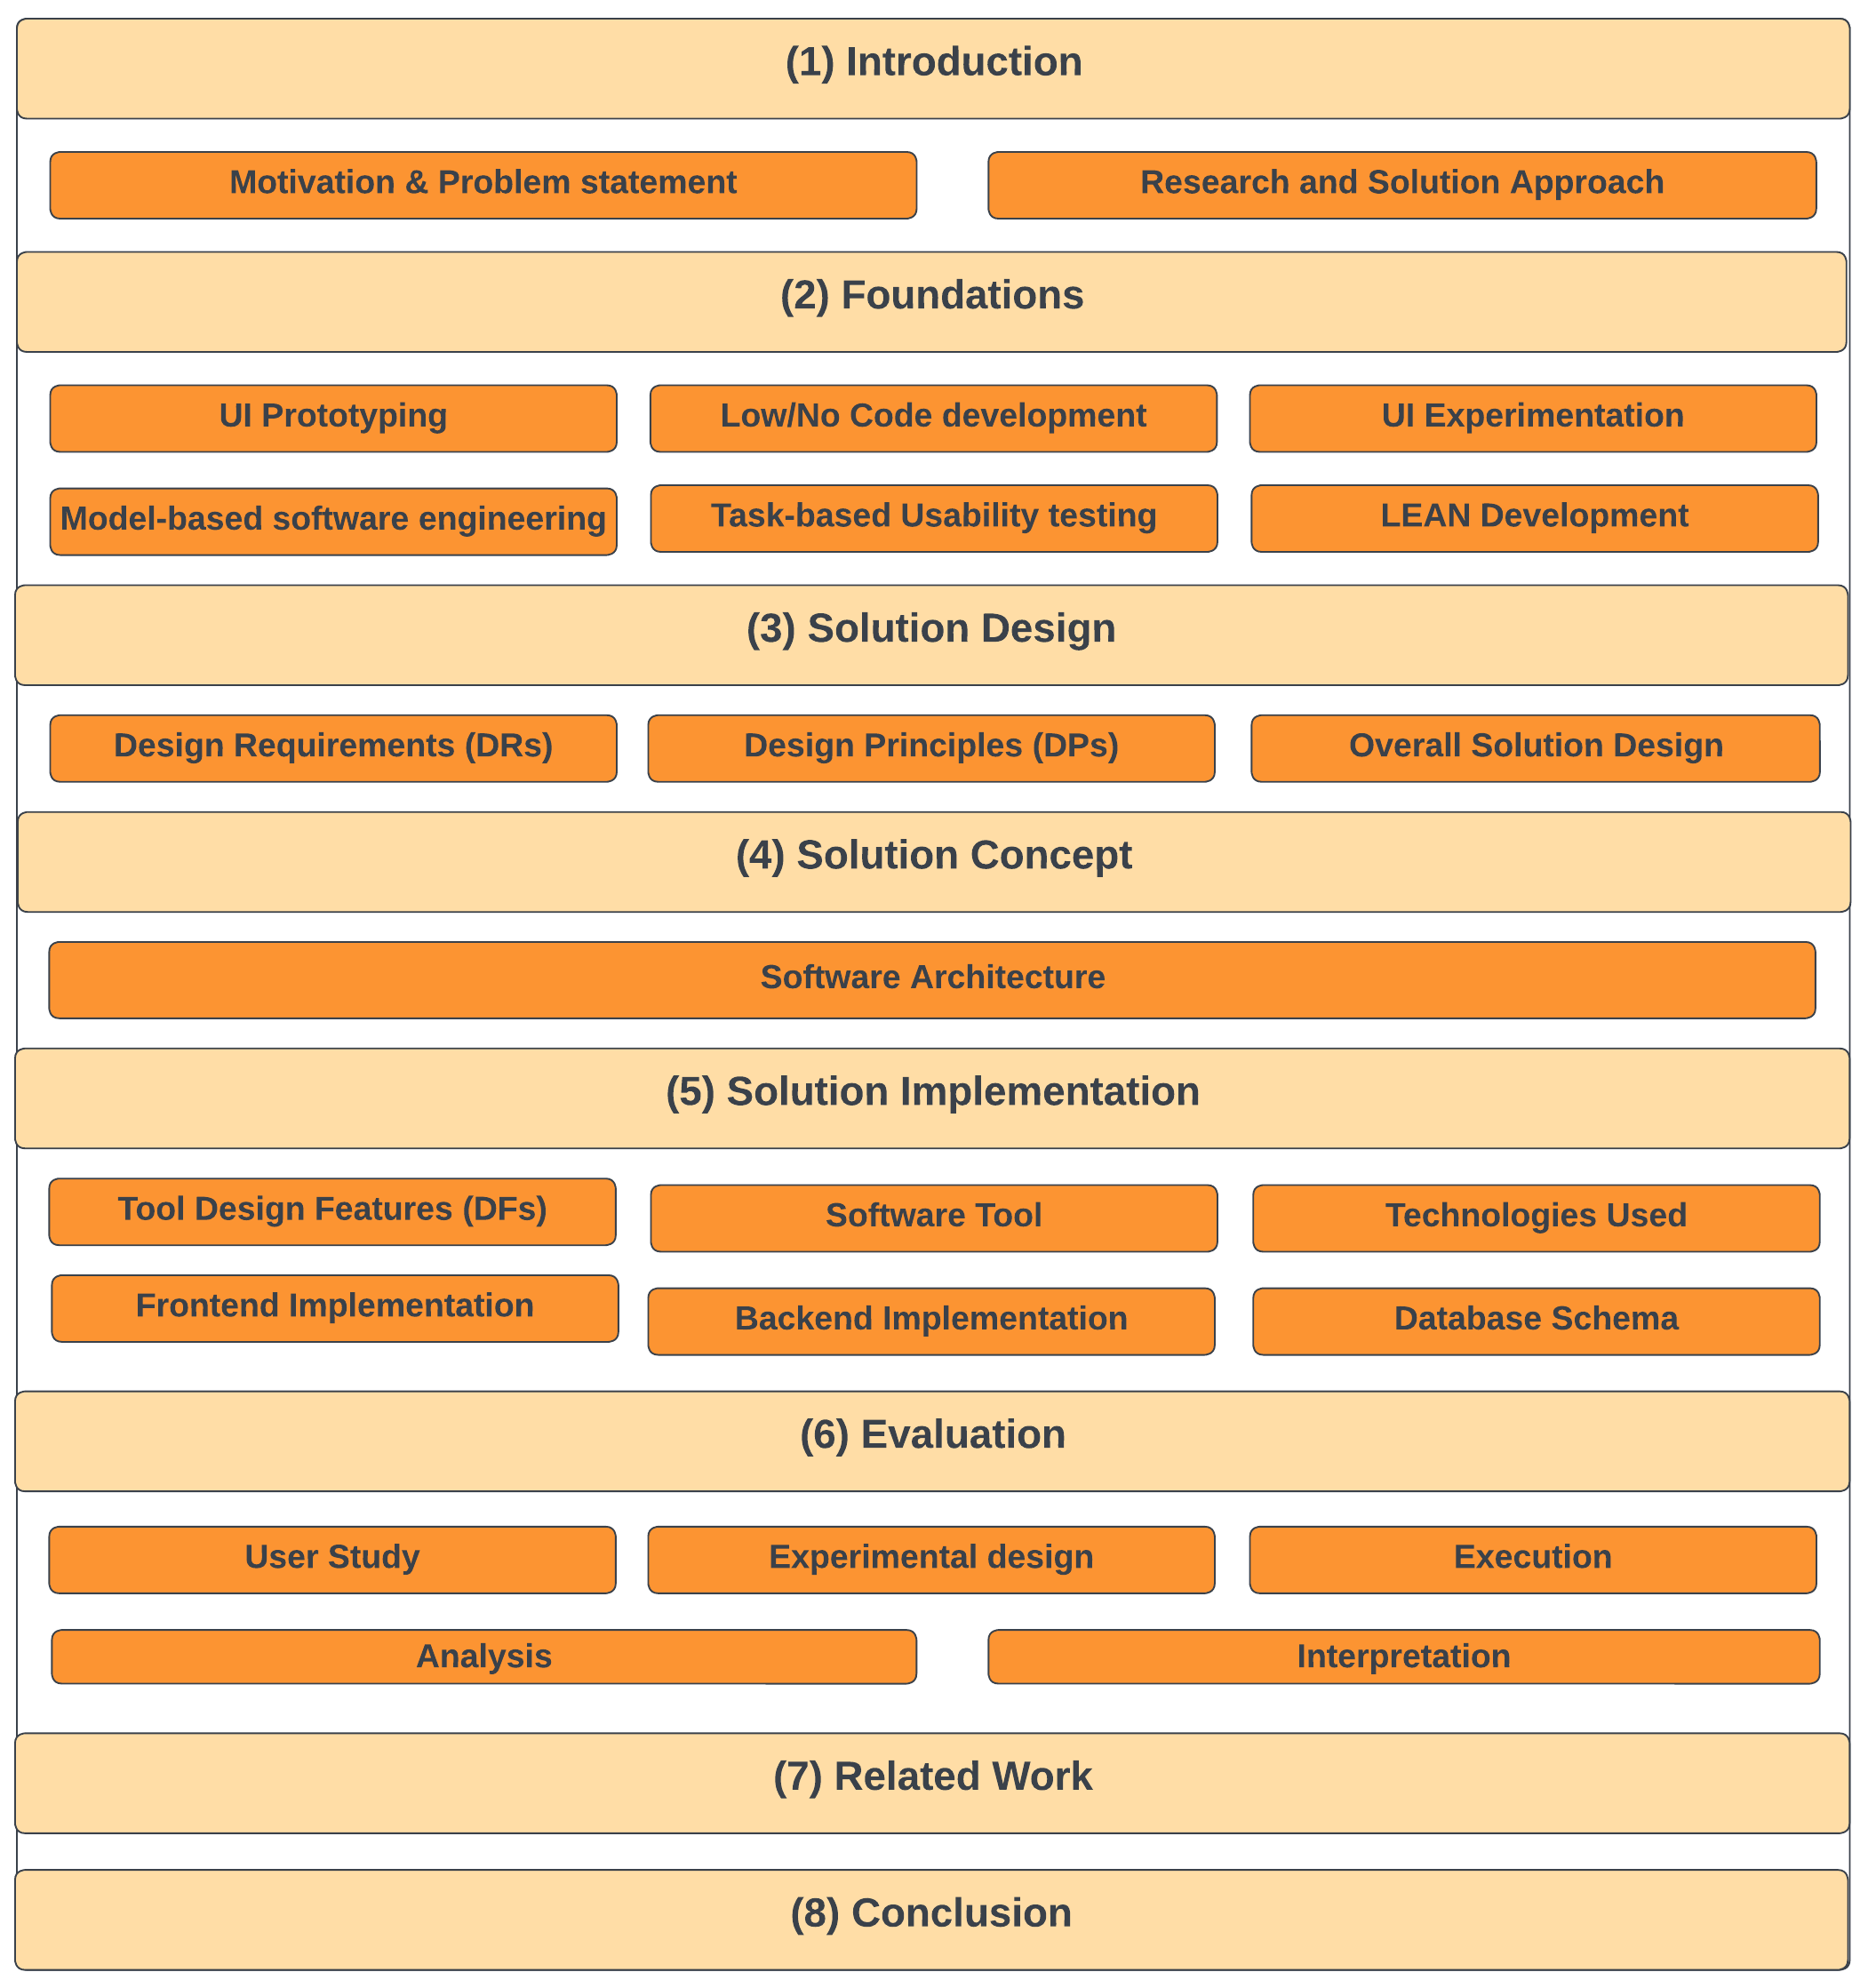
\includegraphics[scale=0.2]{Structure.png}
    \caption{Thesis Structure}
    \label{intro:fig:structure}
\end{figure}

Next, the \textit{\hyperref[chap:foundations]{(2) Foundations}} chapter is used to gain the knowledge required to understand the scope of our work, which includes UI prototyping, low/no code development, model-based software engineering, task-based usability testing, UI experimentation, and LEAN development.
The \textit{\hyperref[chap:design]{(3) Solution Design}} chapter outlines the design requirements, design principles, and overall solution design. 
Similarly, the \textit{\hyperref[chap:concept]{(4) Solution Concept}} chapter presents the software architecture, UI prototype management, UI experimentation management, persistence infrastructure, deployment infrastructure, and security infrastructure.
Next, the \textit{\hyperref[chap:implementation]{(5) Solution Implementation}} chapter provides detailed insights into the tool design features, explains the software tool we developed, technologies used, frontend and backend implementation, and database schema. 
Next, the \textit{\hyperref[chap:evaluation]{(6) Evaluation}} chapter showcases the user study, experimental design, execution, analysis, and interpretation. 
Next, the \textit{\hyperref[chap:relatedWork]{(7) Related Work}} section discusses current tools and state-of-the-art technologies and compares them with our DRs.
Finally, in the \textit{\hyperref[chap:conclusion]{(8) Conclusion}} chapter, we summarize our work, future work, and research contributions.
